\chapter{Context}

\section{What is Android ?}

\section{Presentation of the subject}

\noindent With the Android platform, the developer can have many possibilities in the creation of applications. Therefore there are so many applications available on the Android Market.

\noindent The final purpose of the project is to use more functionnalities as possible in an application to get a view of what is feasible. To save development time, the software (a task manager), realized in the first semester as part of the unit value \textit{Mod�lisation, Interface utilisateur, Conception Avanc�e (MICA)}, was chosen.

\noindent So that, the project consists to :
\begin{itemize}
    \item adapt the existing application to an Android smartphone;
    \item add correctly several useful functionnalities to the smartphone;
    \item have a functionnal application.

\end{itemize}

\section{The task manager}

\subsection{Presentation of existing}

\noindent The task manager realized as part of the unit part MICA\protect\footnote{Mod�lisation, Interface utilisateur, Conception Avanc�e} is a sofware for managing daily tasks that everyone should make. It is a memory aid used by everyone.

\subsubsection{Existing functionnalities}

\noindent This software can realize the following actions : 
\begin{itemize}
    \item manage tags;
    \item manage tasks;
    \item sort tasks according to specific criteria;
    \item assign sub-tasks to tasks;
    \item change language via a software internationalization in English;
    \item save the tasks list.

\end{itemize}

\subsubsection{View of the existing}

\begin{figure}[!ht]
        \centering
        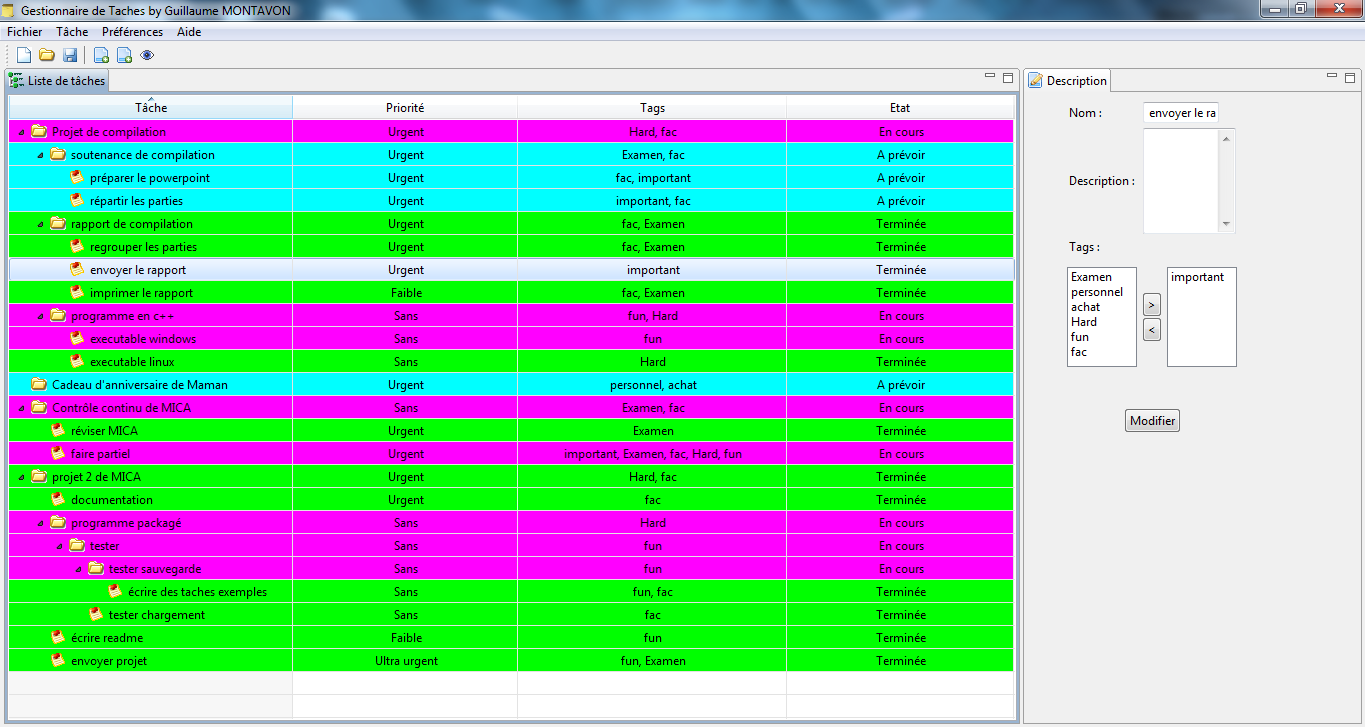
\includegraphics[width=13cm,height=8cm]{gestionnaireTacheExistantGuillaume.png}
        \caption{Example of screenshot of the existing task manager}

\end{figure}


\subsection{Presentation of the software for smartphones}

\noindent The sofware must be able to adapt to a smartphone while containing the functionnalities listed above. That is to say, he must be able to adapt to screen size, have a simple interface and not over-elaborate, but still full. It must also include new possibilities available with Android.

\noindent Omitting the functionnalities already listed in the presentation of the existing, the task manager for smartphone must be able to :
\begin{itemize}
    \item use the SQLite database available on Android smartphones;
    \item synchronize with a remote server;
    \item use the various functionnalities included with Android;
    \item manage user accounts on the server.

\end{itemize}

\section{Specifications}

\subsection{Application design}

\noindent The application can be divided into different main parts.
One general part that reflects the objectives of the first software task manager.
One part concerning the storage of information on the smartphone.
And a last part to manage the remote server.

\noindent The general objectives of the application are :
\begin{itemize}
    \item manage the application with tasks and tags (added, remove, modification, sorting);
    \item a graphical interface fluid and pleasant to use while still powerfull and complete;
    \item internationalization of the application in English;
    \item manage the application preferences.

\end{itemize}

\vspace{1cm}

\noindent Concerning the database :
\begin{itemize}
    \item creation of a coherent basis to manage all the data of the application;
    \item storing, modifying and deleting data.

\end{itemize}

\vspace{1cm}

\noindent Concerning the synchronization with the remote server :
\begin{itemize}
    \item creation of a database more evolved than the smartphone;
    \item sending and receiving data with their storage, modification and deleting;
    \item manage users;
    \item implementation of various methods of synchronization :
    \begin{itemize}
        \item overwrite data from the smartphone replaced by those of the server;
        \item overwrite data from the server replaced by those of the smartphone;
        \item combine data of the server and the smartphone.

    \end{itemize}
    \item manage a proxy server.

\end{itemize}

\subsection{Technical constraints}

\noindent Developing an application with Android imposes some constraints to have a result.

\subsubsection{Development tools}

\noindent Several tools are available to easily develop with Android :
\begin{itemize}
    \item Google Android SDK\protect\footnote{Software Development Kit} which contains an emulator of smartphone;
    \item eclipse IDE\protect\footnote{Integrated Development Environment} to develop in Java;
    \item Android plugin ADT which one can to use the emulator with eclipse.

\end{itemize}


\subsubsection{Web server}

A web server was set up to test remote synchronization. This server is hosted by \textit{OLikeOpen} (web host which offer his services for free) and has a MySQL database and PHP tools for communicating with it.

\subsubsection{Miscellaneous}

There are lot of release of Android and they evolve everyday, so this is why the development was completed and tested on 2.2 release (\textit{FroYo}).
However, an emulator is not sufficient to verify the correct running of the application, a smartphone that has the correct release of Android was necessary to validate the tests.

\subsection{Temporal constraints}

The first part of the project consists to the study of the Android platform, so the development time of the application depends of time to get one's feet wet with the tools proposed by Android.
The rest of the time is a full development of the task manager.

\clearpage
